%%%%%%%%%%%%%%%%%%%%%%%%%%%%%%%%%%%%%%%%%%%%%%%%%%%%%%%%
% IE643 course poster, A1 portrait, original template colours.
% Layout, class, header, framed two-column body and section order follow the course template
% (a0poster class by Kettl and Weiser, CC BY-NC-SA 3.0; design: Timothy Kodikara).
% Compile (twice) with:  pdflatex IE643_Poster.tex
%%%%%%%%%%%%%%%%%%%%%%%%%%%%%%%%%%%%%%%%%%%%%%%%%%%%%%%%
%----------------------------------------------------------------------------------------
%	PACKAGES AND OTHER DOCUMENT CONFIGURATIONS
%----------------------------------------------------------------------------------------
\documentclass[a1,portrait]{a0poster}
%%
\usepackage[top=3.5cm, bottom=0.3cm, left=3.5cm, right=2cm]{geometry}
\usepackage[compact]{titlesec}
\usepackage{multicol} % This is so we can have multiple columns of text side-by-side
\columnsep=70pt % This is the amount of white space between the columns in the poster
\columnseprule=10pt % This is the thickness of the blue line between the columns in the poster
\usepackage[svgnames]{xcolor}
\usepackage{palatino} % Palatino font, as in the template
\usepackage{xkeyval}
\usepackage{graphicx} % Required for including images
\setlength{\abovecaptionskip}{5pt plus 5pt minus 3pt}
\graphicspath{{figures/}} % Location of the graphics files
\usepackage{booktabs} % Top and bottom rules for table
\usepackage[font=small,labelfont=bf]{caption} % Required for specifying captions to tables and figures
\usepackage{amsfonts, amsmath, amsthm, amssymb} % For math fonts, symbols and environments
\usepackage{csquotes}
\usepackage{wrapfig} % Allows wrapping text around tables and figures
\usepackage{multirow}
\usepackage{makecell}
\usepackage{array}
\def\columnseprulecolor{\color{NavyBlue}}%
\usepackage{framed}
\colorlet{frameborder}{NavyBlue}
%----------------------------------------------------------------------------------------
%	POSTER HEADER
%----------------------------------------------------------------------------------------
% The header is divided into three boxes:
% The widths of these boxes can be easily edited to accommodate your content as you see fit
\begin{document}
\begin{minipage}[c]{\linewidth}
\vspace{0.1cm}
\noindent\makebox[\textwidth][c]{
\begin{minipage}[c]{0.14\linewidth}
\vspace{0pt}\raggedright
\hspace{1cm}

\includegraphics[scale=1.3,width=\linewidth]{figures/logo.png}
\end{minipage}
\hfill
\begin{minipage}[c]{0.75\textwidth}
\centering
\Huge \color{Green} \textbf{IE643 Course Project}\\[0.4cm]
\Huge \color{NavyBlue} \textbf{Constraint-Driven Multimodal Diffusion\\ using Text, Sketch and Reference Image}\\[0.4cm]
\Large \color{NavyBlue} \textbf{Team: One Sheep Army}\\[0.4cm]
\large \color{Black} \textbf{[Team Member Name 1 $^{1}$ (Roll Number), Team Member Name 2 $^{2}$ (Roll Number)]}\\[0.2cm] % Author(s): FILL IN
\small \text{[XXXX@iitb.ac.in$^{1}$, XXXXX@iitb.ac.in$^{2}$]}\\
\end{minipage}
\begin{minipage}[c]{0.145\textwidth}
\vspace{0pt}\raggedleft

\includegraphics[scale=1.3,width=\linewidth]{figures/IE643-Logo.pdf}
\hspace{1cm}
\end{minipage}}
\\[0.1cm]%
% A bit of extra whitespace between the header and poster content
%----------------------------------------------------------------------------------------
\color{NavyBlue}\setlength\FrameRule{18pt}
\begin{framed}
\vspace{0.4cm}
\begin{multicols}{2} % a portrait poster is split into 2 columns
%----------------------------------------------------------------------------------------
%	Abstract
%----------------------------------------------------------------------------------------
\color{Black}
\section*{Abstract}
Text, sketch and reference image can disagree about the same object. We study an \textbf{Attribute Routing Layer (ARL)} that gives each modality an explicit job: \textbf{text $=$ identity}, \textbf{sketch $=$ shape}, \textbf{reference $=$ colour and material}. The ARL is meant to sit between the three conditioning signals and a frozen SDXL + ControlNet + IP-Adapter backbone. We tested routing variants on a 200-photo Sketchy conflict set. \textbf{Detecting conflicts and rescaling global strengths did not enforce attribute control.} A neutral-caption intervention improved object compliance and sketch fidelity, but not colour or material.

%----------------------------------------------------------------------------------------
%	INTRODUCTION
%----------------------------------------------------------------------------------------
\section*{Introduction}
\begin{itemize}
	\item One generation receives text, sketch and reference at once, and they can conflict: the caption says \emph{purple}, the reference is \emph{silver}.
	\item Without a rule the strongest pathway wins; a reference also carries its own object shape.
	\item A \textbf{separate attribute responsibility} per modality makes the conflict well-posed and measurable per attribute.
	\item Rule used: where inputs conflict, \textbf{the reference wins colour}.
\end{itemize}

%----------------------------------------------------------------------------------------
%	Main Contributions
%----------------------------------------------------------------------------------------
\section*{Main Contributions}
\begin{itemize}
	\item \textbf{Three-modality attribute-routing formulation:} each attribute has exactly one governing modality.
	\item \textbf{Attribute Routing Layer} architecture that directs identity, geometry and appearance to separate pathways of SDXL.
	\item \textbf{Conflict-oriented dataset:} Sketchy-based, with object, colour, material and swapped-reference conflict rows.
	\item \textbf{Experiments on attribute-level control}, including negative results, with attribute-wise compliance metrics.
\end{itemize}

%----------------------------------------------------------------------------------------
%	Workflow
%----------------------------------------------------------------------------------------
\color{Black}
\section*{Workflow}
Figure \ref{workflow} illustrates the workflow, from the three inputs to attribute-wise evaluation.
\begin{center}
	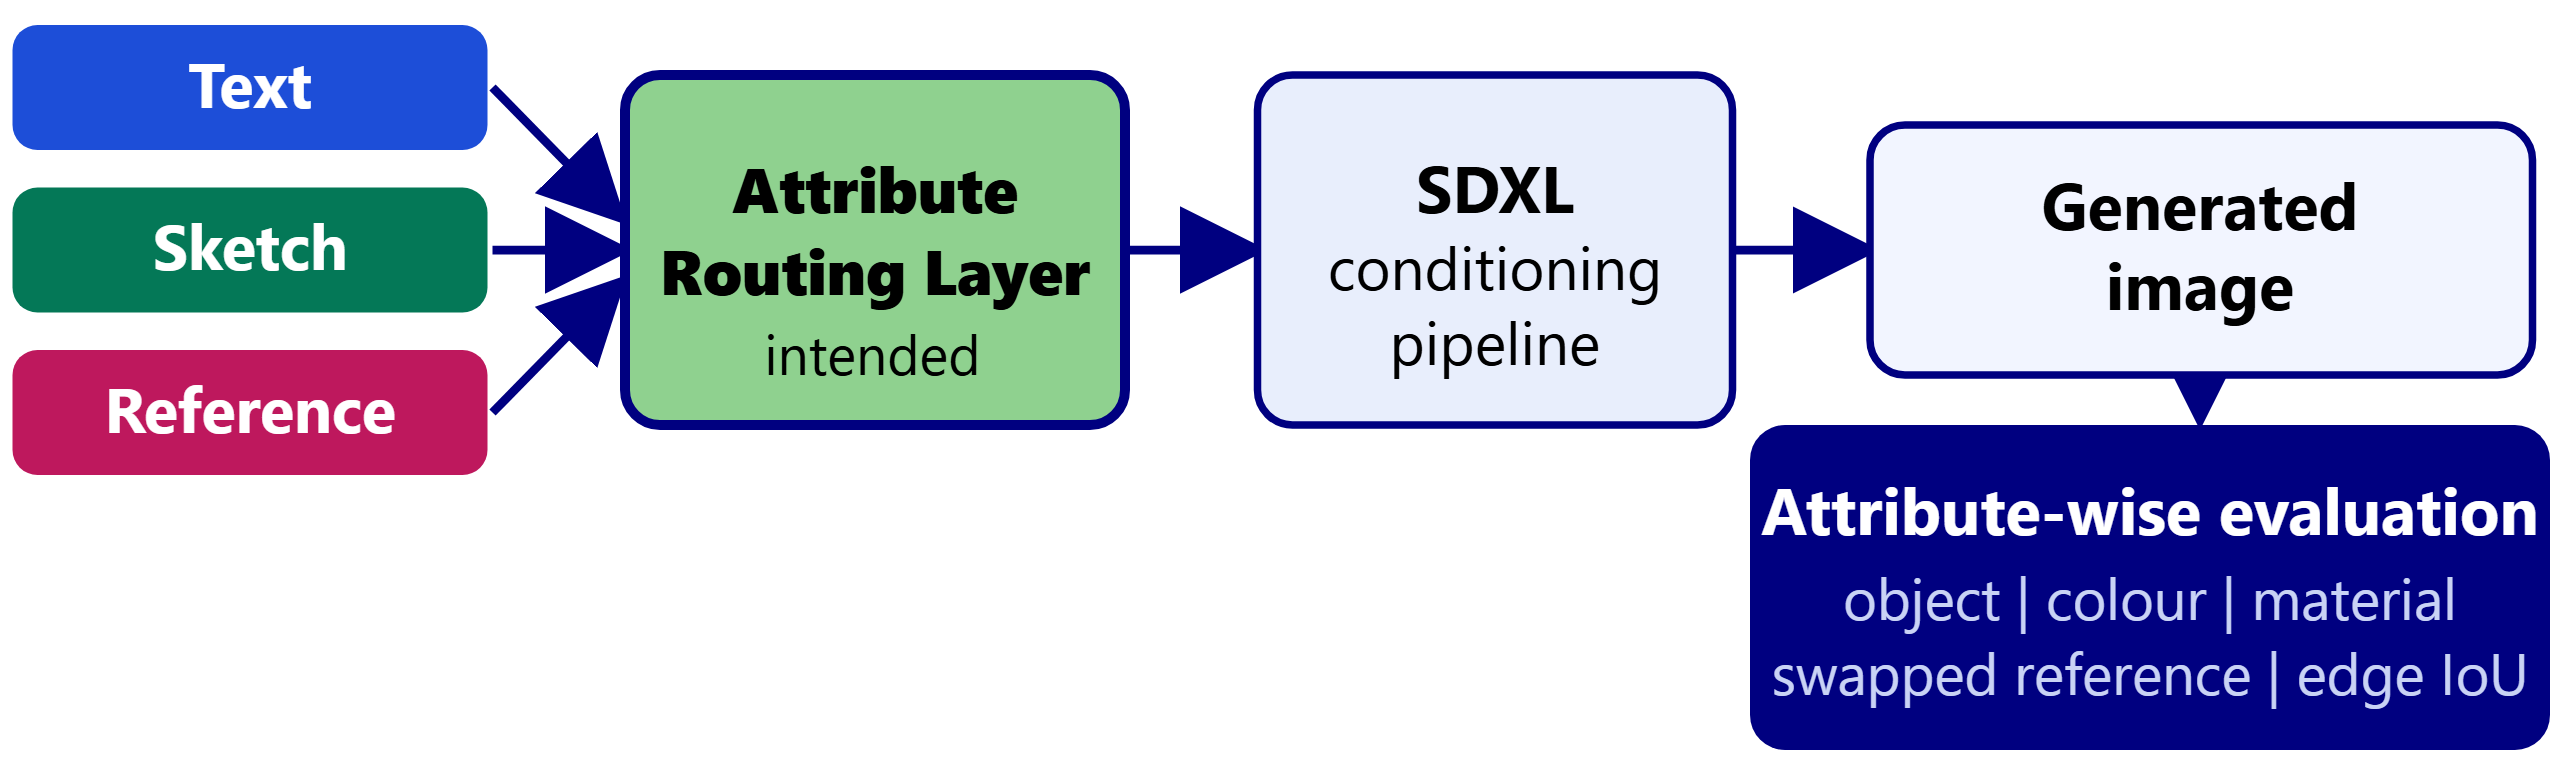
\includegraphics[width=0.95\linewidth]{figures/Workflow.png}
	\captionof{figure}{\color{Blue} Overall Workflow}
	\label{workflow}
\end{center}

%----------------------------------------------------------------------------------------
%	Methodology
%----------------------------------------------------------------------------------------
\section*{Methodology}
Figure \ref{method} contrasts the fixed-strength baseline with the proposed routing; Figure \ref{Arch} shows the full architecture.
\begin{center}
	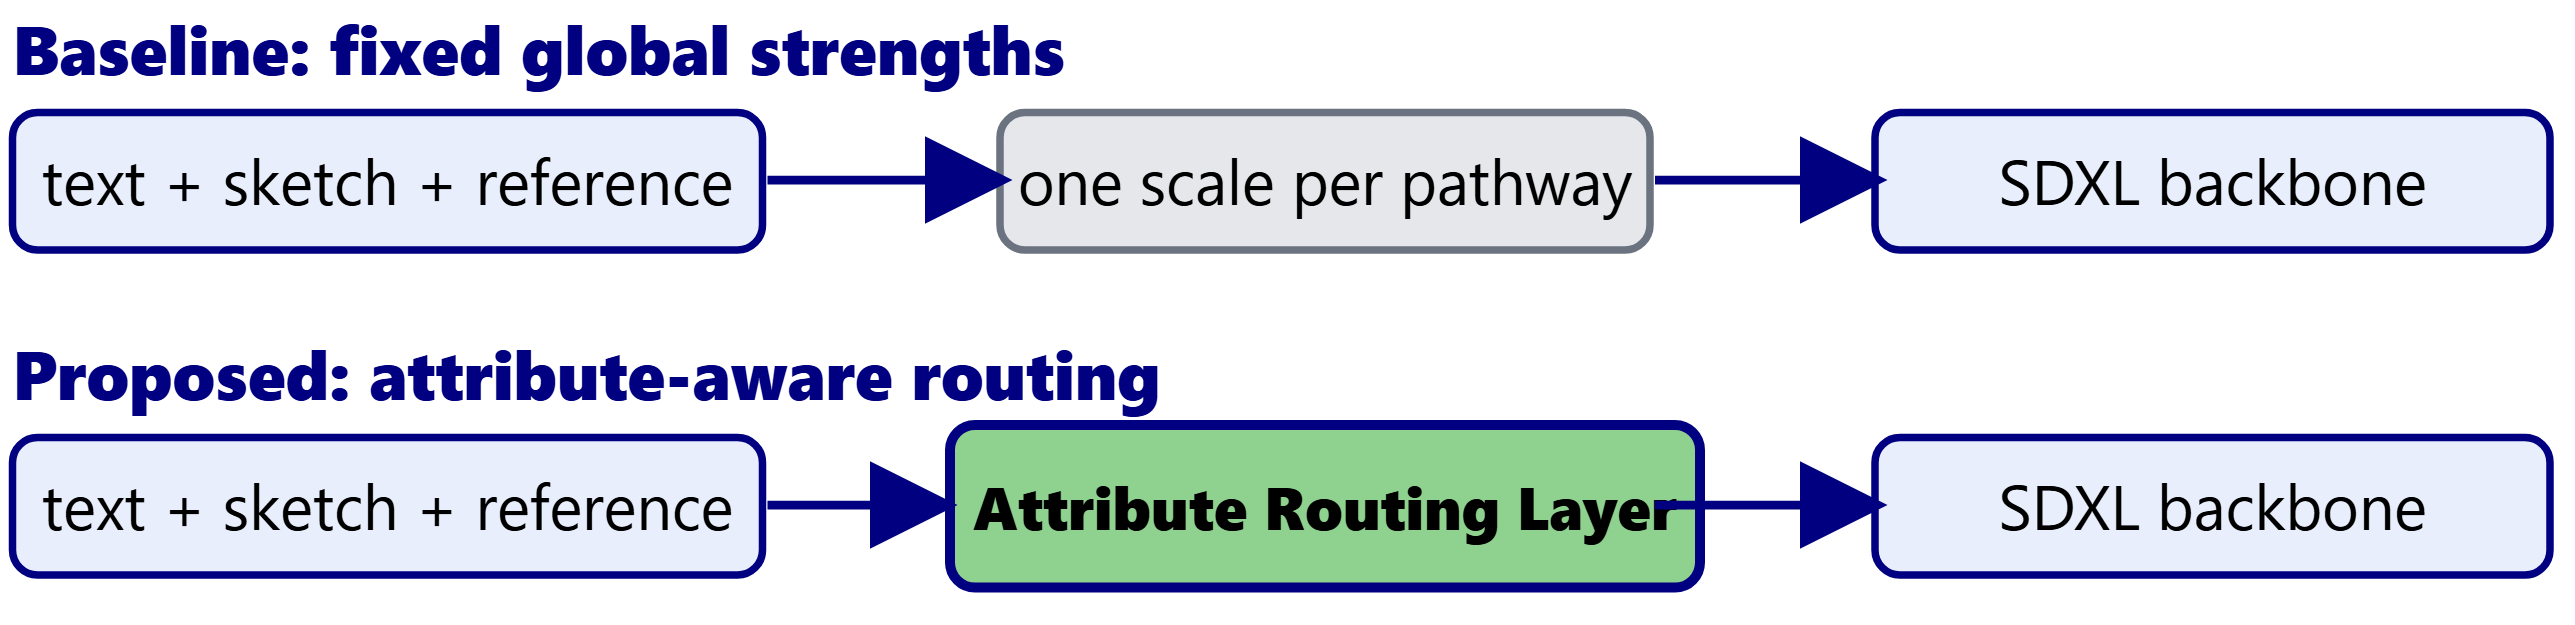
\includegraphics[width=0.95\linewidth]{figures/Methodology.png}
	\captionof{figure}{\color{Blue} Baseline versus attribute-aware routing}
	\label{method}
\end{center}
\vspace{-\baselineskip}
\begin{itemize}
	\item \textbf{Backbone:} frozen SDXL, scribble ControlNet (sketch), IP-Adapter ViT-H (reference).
	\item \textbf{Router:} reads the three inputs and decides, per attribute, which pathway may carry it.
	\item \textbf{Conditioning pathways:} text cross-attention (identity), ControlNet residuals (geometry), IP-Adapter tokens (colour, material).
	\item \textbf{Intervention tested:} neutral caption (colour words $\rightarrow$ ``colored'', material words $\rightarrow$ ``solid'') plus a higher IP-Adapter scale.
\end{itemize}

\columnbreak
%----------------------------------------------------------------------------------------
%	Architecture Diagram
%----------------------------------------------------------------------------------------
\color{Black}
\section*{Architecture: Attribute Routing Layer}
\begin{center}
	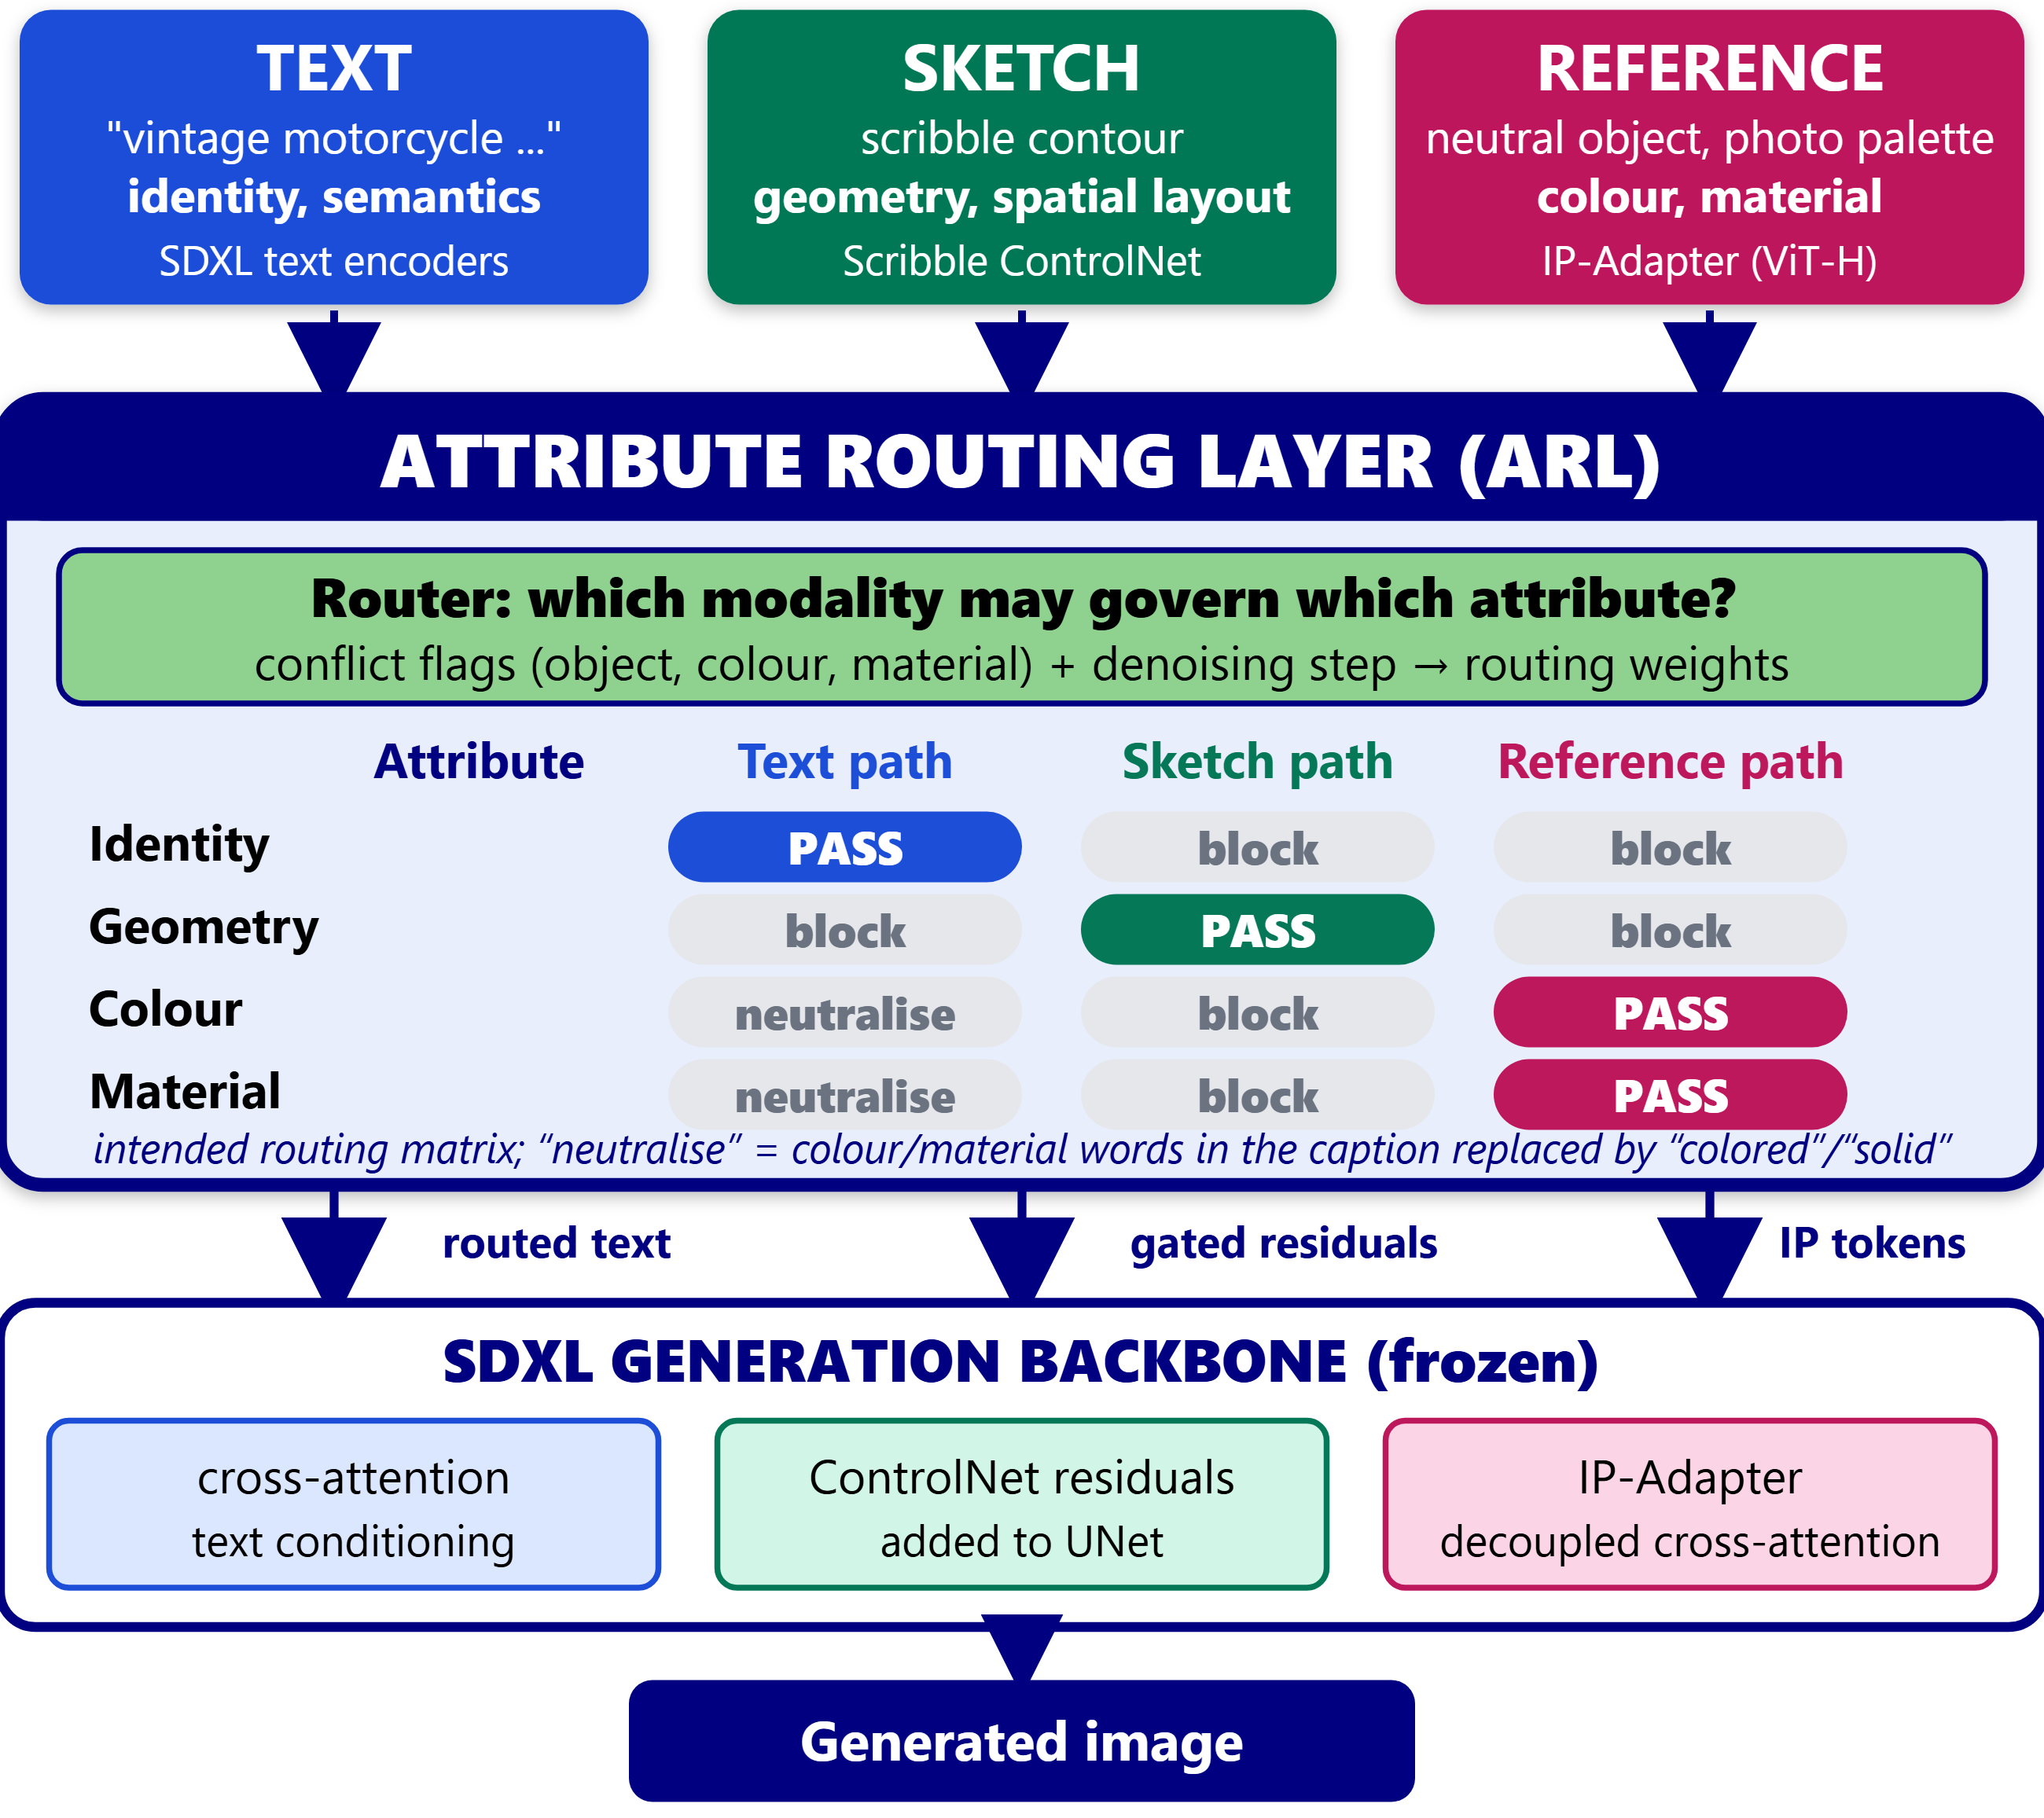
\includegraphics[width=0.97\linewidth]{figures/Architecture.png}
	\captionof{figure}{\color{Blue} The ARL sits between the three conditioning pathways and frozen SDXL (\textbf{intended} routing).}
	\label{Arch}
\end{center}
\vspace{-0.5\baselineskip}
\noindent{\color{Red}\fbox{\parbox{0.95\linewidth}{\small \textbf{Demonstrated:} rule-based text-path neutralisation, conflict flags. \textbf{Not demonstrated:} learned routing that reliably enforces colour and material from the reference. Attribute-level control is \textbf{not solved}.}}}

%----------------------------------------------------------------------------------------
%	Dataset Details and Experimental Setup
%----------------------------------------------------------------------------------------
\color{Black}
\section*{Dataset Details}
Sketchy sketch-photo pairs; about 200 selected photos, one object each. Each example has a photo, sketch, Qwen3-VL-2B caption and a neutral-object reference carrying the photo's colour, material and finish. Conflict cases: object, colour, material and swapped reference (rows built from metadata).
\begin{center}
	\begin{tabular}{|l|c|c|c|c|}
		\hline
		Split & Train & Validation & Test & Total\\
		\hline
		Photos & 160 & 20 & 20 & \textbf{200}\\
		\hline
	\end{tabular}
	\captionof{table}{\color{Blue} Split by photo.}
\end{center}

%----------------------------------------------------------------------------------------
%	Novelty Assessment
%----------------------------------------------------------------------------------------
\color{Black}
\section*{Novelty Assessment}
Experiments run to investigate the architecture:
\begin{center}
\small
\renewcommand{\arraystretch}{1.25}
\begin{tabular}{|p{0.2\linewidth}|p{0.3\linewidth}|p{0.42\linewidth}|}
\hline
\textbf{Approach} & \textbf{What was tested} & \textbf{Key observation}\\
\hline
Fixed / scheduled conditioning & Constant or time-scheduled sketch, reference and text strengths & Reference copies its own object; no attribute separation\\
\hline
Learned global router & CLIP compatibility scores $\rightarrow$ 4 global strengths & No better than the hand schedule; blind to colour and material conflicts\\
\hline
Governance conflict detection & Network flags object, colour, material conflicts & Detects conflicts well (colour 0.755, material 0.940), yet images barely changed\\
\hline
Role gates and neutral caption & Per-role gates in SDXL; colour and material words neutralised & Gates moved little; neutral caption improved sketch fidelity and object compliance\\
\hline
Colour adapter and role LoRA & Palette adapter; role-specific LoRA & LoRA raised edge overlap but severely cut target similarity\\
\hline
\end{tabular}
\captionof{table}{\color{Blue} Summary of experiments.}
\end{center}
\textbf{Key lesson:} detecting conflicts and adjusting \emph{global} strengths does not enforce \emph{attribute-specific} control; sketch fidelity, reference compliance and target similarity trade off.

%----------------------------------------------------------------------------------------
%	Results
%----------------------------------------------------------------------------------------
\color{Black}
\section*{Results}
\begin{center}
	\scalebox{0.85}{
		\begin{tabular}{|l|c|c|c|c|c|}
			\hline
			Method & Object & Colour & Material & Swapped ref. & Edge IoU\\
			\hline
			Fixed baseline & 0.10 & \textbf{0.70} & \textbf{0.67} & \textbf{0.70} & 0.213 \\
			Neutral caption + IP scale 1.0 & 0.30 & \textbf{0.70} & \textbf{0.67} & 0.00 & 0.376 \\
			Role LoRA & 0.30 & 0.30 & 0.00 & 0.40 & \textbf{0.753} \\
			\hline
		\end{tabular}
	\label{table}}\\
\captionof{table}{\color{Blue} Compliance rates and edge IoU, verified 12-test-photo comparison.}
	\vspace{-0.25in}
\end{center}
\vspace{0.25in}
Table \ref{table} shows that the neutral-caption intervention improved object compliance and sketch fidelity but did not improve colour or material compliance, and failed on swapped references (0.00 vs 0.70). Role LoRA improved edge overlap but suffered a severe target-similarity drop.
\begin{center}
	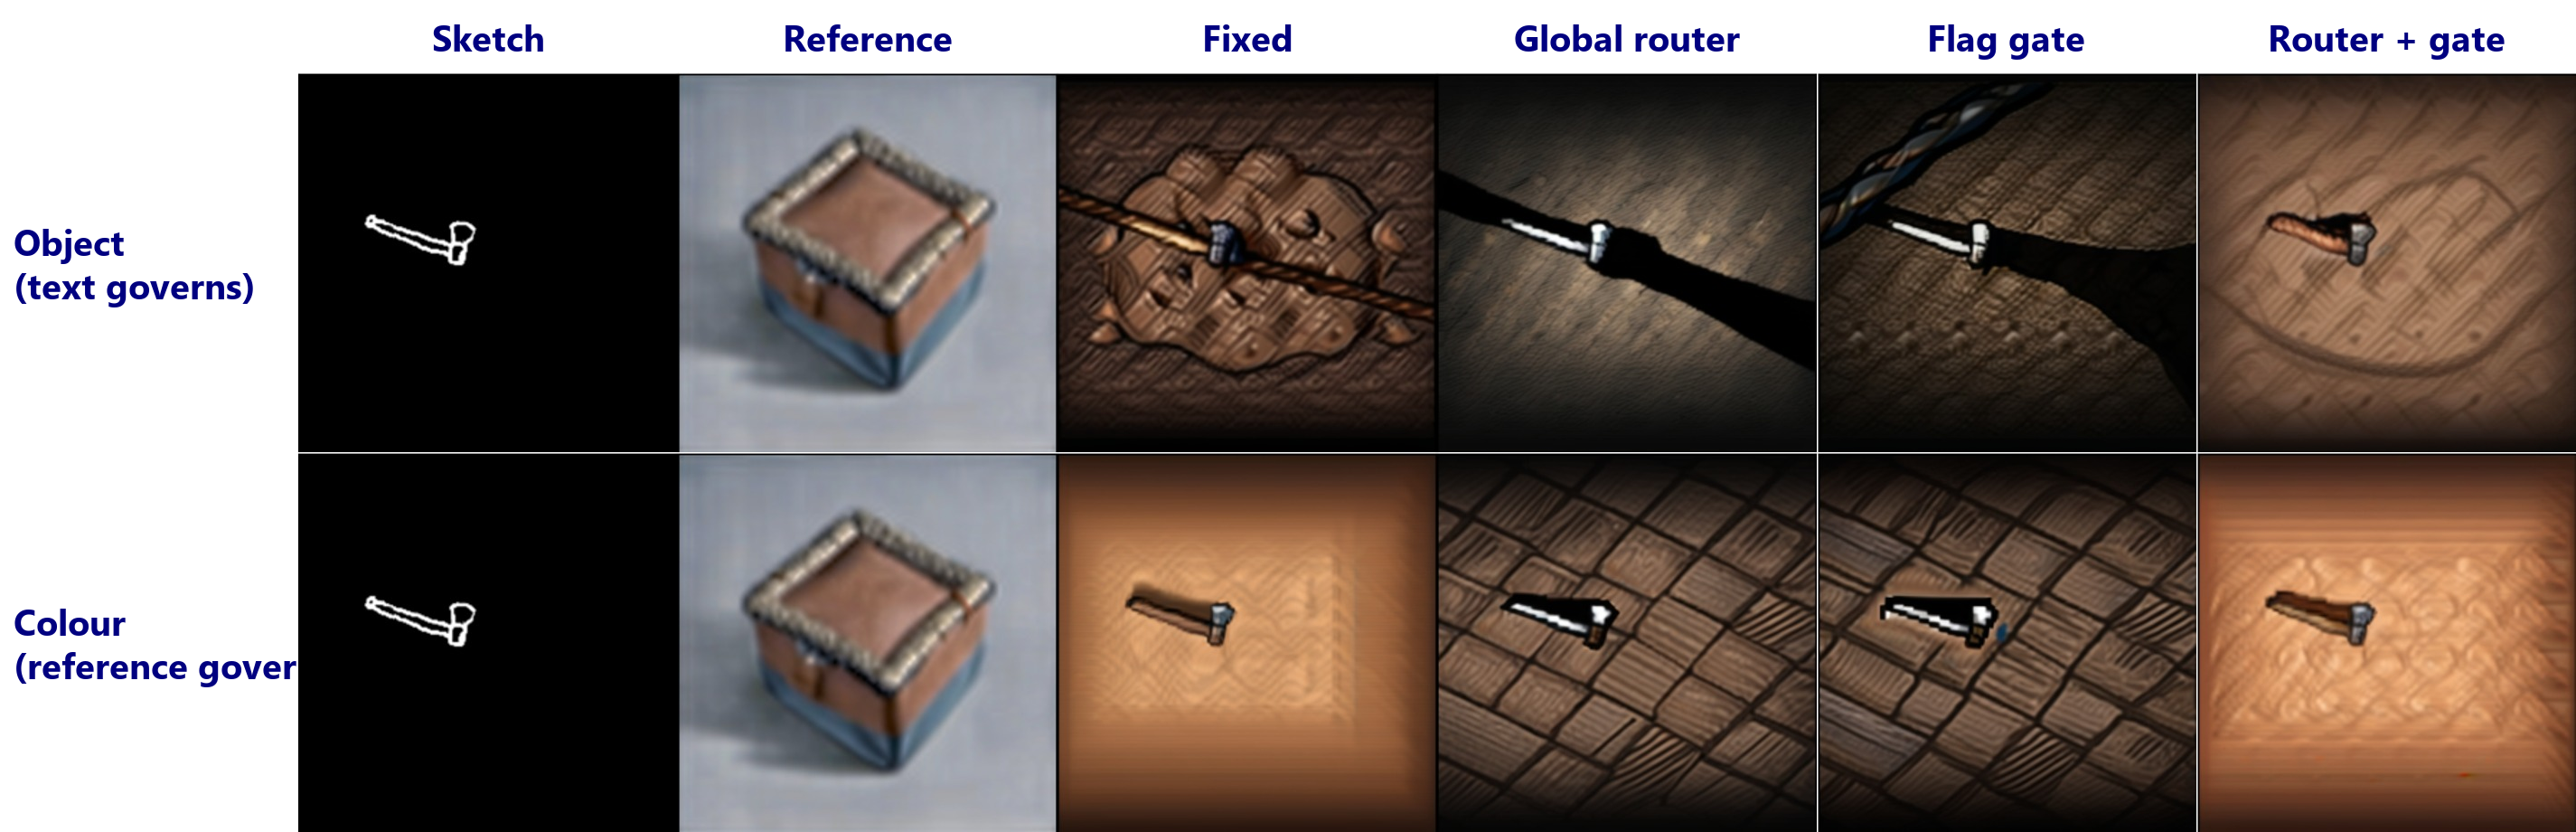
\includegraphics[width=0.97\linewidth]{figures/Qualitative.png}
	\captionof{figure}{\color{Blue} Pilot rows (earlier global-conditioning arms, one test photo). Sketch shape is followed in all arms; the caption's object is never produced (object conflict: failure); the brown leather palette follows the reference (colour: success). \textbf{[PLACEHOLDER: qualitative images for the three methods of Table \ref{table} were not in the project files; insert here.]}}
\end{center}

%----------------------------------------------------------------------------------------
%	CONCLUSIONS
%----------------------------------------------------------------------------------------
\color{Black}
\section*{Conclusion}
\begin{itemize}
	\item Explicit attribute responsibilities (text $=$ identity, sketch $=$ shape, reference $=$ colour and material) make multimodal conflicts well-defined and measurable.
	\item Global conditioning cannot enforce them: flags and strengths changed little in the output.
	\item Reliable attribute-level control with a trained ARL remains open.
\end{itemize}
%----------------------------------------------------------------------------------------
%	References
%----------------------------------------------------------------------------------------
\begin{thebibliography}{6}

\bibitem {SDXL}
Podell, D., et al.: SDXL: Improving latent diffusion models for high-resolution image synthesis. ICLR (2024)

\bibitem {CN}
Zhang, L., Rao, A., Agrawala, M.: Adding conditional control to text-to-image diffusion models. ICCV (2023)

\bibitem {IPA}
Ye, H., et al.: IP-Adapter: Text compatible image prompt adapter for text-to-image diffusion models. arXiv:2308.06721 (2023)

\bibitem {Sketchy}
Sangkloy, P., et al.: The Sketchy Database: Learning to retrieve badly drawn bunnies. ACM Transactions on Graphics 35(4) (2016)

\bibitem {CLIP}
Radford, A., et al.: Learning transferable visual models from natural language supervision. ICML (2021)

\end{thebibliography}
%----------------------------------------------------------------------------------------
%	ACKNOWLEDGEMENTS
%----------------------------------------------------------------------------------------
\section*{Acknowledgments}
\small \textnormal{We thank \textbf{[FILL IN: acknowledgements]}}

\section*{Github Link and Demo Video Link}
\vspace{-0.5cm}

\begin{center}
		\begin{minipage}{0.4\linewidth}
			\centering
			\textbf{Github Repository}\\[1ex]
			
\includegraphics[width=0.5\linewidth]{Repo_QR.png}\\[0.5ex]
			\scriptsize github.com/Harshitha-282007/constraint-driven-multimodal-diffusion
		\end{minipage}\hfill
		\begin{minipage}{0.4\linewidth}
			\centering
			\textbf{Demo Video Link}\\[1ex]
			\fbox{\parbox[c][0.5\linewidth][c]{0.5\linewidth}{\centering\small [PLACEHOLDER: demo link not available]}}
		\end{minipage}
\end{center}


\end{multicols}
\vspace{0.4cm}
\end{framed}
\end{minipage}
\end{document}
%----------------------------------------------------------------------------------------
%%%%%%%%%%%%%%%%%%%%%%%%%%%%%%%%%%%%%%%%%%%%%%%%%%%%%%%%
